\section{Rounding the Linear Program}

We will now develop an algorithm for rounding a solution $x$ to the metric LP relaxation~\ref{eq:metric-lp}. Let's start by addressing how to construct a \emph{valid} multicut, then determine how to make it \emph{low-cost}. For the remainder of these notes, we'll denote $d_x(u, v)$ as the metric completion of $x$ on edge $(u, v)$.

% --------------------------------------------------------------------
% BALLS AND PIPE SYSTEMS
% --------------------------------------------------------------------

\subsection{Balls and Pipe Systems}

We want to leverage the metric structure from our LP relaxation to construct our multicut. One way to do this is to partition the graph into clusters separating each $s_i, t_i$ pair, then remove the multicut consisting of edges that cross the boundary of each cluster. We can use the fact that $d_x$ is a metric to construct our clusters by choosing balls of a certain radius as measured by $d_x$. Let's define the ball of radius $r$ centered at vertex $u' \in V$ as $\mathcal{B}_x(u', r) \subseteq V$, the set of all vertices within distance $r$ of $u'$ as measured by the distance $d_x$.
\begin{equation*}
\mathcal{B}_x(u', r) = \{ v \in V : d_x(u', v) \leq r \}
\end{equation*}

Later on, it will be useful for us to consider the \emph{volume} of each ball. Given $S \subseteq V$, let $E(S)$ denote the set of edges whose endpoints are contained in $S$. Additionally, let $\partial(S)$ denote the set of edges on the \emph{boundary} of $S$, i.e. $(u, v)$ with $u \in S$ and $v \notin S$. The volume of a ball $\mathcal{B}_x(u', r)$ is defined by the following:
\begin{equation*}
\text{Vol} \; \mathcal{B}_x(u', r)
= \sum_{e \in E(\mathcal{B}_x(u', r))} c_e x_e + \sum_{(u, v) \in \partial(\mathcal{B}_x(u', r)) : u \in \mathcal{B}_x(u', r)} c_{uv} \big( r - d_x(u', u) \big)
\end{equation*}

Williamson and Shmoy's \emph{The Design of Approximation Algorithms} uses the analogy of a \emph{pipe system} to interpret these definitions. We think of the graph as a network of pipes: each edge $e$ is replaced with a pipe of \emph{length} $x_e$ and \emph{cross sectional area} $c_e$. The term $c_e x_e$ then denotes the volume of the pipe replacing $e$. The quantity $\text{Vol} \; \mathcal{B}_x(u, r)$ could then be interpreted as the total volume of all pipes within a radius $r$ of $u$.
\begin{equation*}
\text{Vol} \; \mathcal{B}_x(u', r)
= \underbrace{\sum_{e \in E(\mathcal{B}_x(u', r))} c_e x_e}_\text{Total volume of pipe contained in the ball}
+ \underbrace{\sum_{(u, v) \in \partial(\mathcal{B}_x(u', r)) : u \in \mathcal{B}_x(u', r)} c_{uv} \big( r - d_x(u', u) \big)}_\text{Volume of pipe contained within the boundary}
\end{equation*}

To visualize the second sum, consider the following diagram
\begin{figure}[h!]
    \centering
    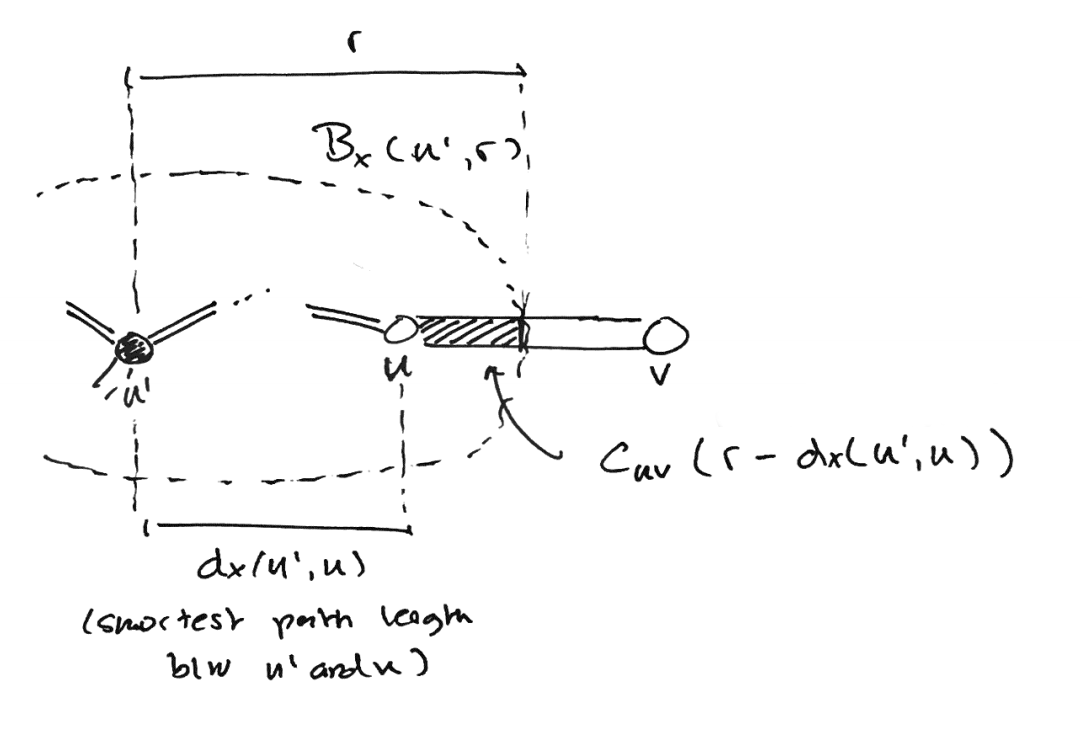
\includegraphics[scale=0.17]{images/image-4.png}
\end{figure}

% --------------------------------------------------------------------
% ROUNDING VIA BALLS
% --------------------------------------------------------------------

\subsection{Rounding via Balls}

Our rounding algorithm will cluster the graph according to appropriately chosen balls. All that remains is to choose the center and radius for each ball. These values will need to be chosen such that each $s_i, t_i$ pair is separated. A certain method of ensuring separation is to center a ball at each $s_i$, then set each radius to $r = 0$. $\mathcal{B}_x(s_i, 0)$ is always the singleton containing $s_i$ thus $s_i$ and $t_i$ are always separated. On the other hand, the ball centered at $s_i$ and with too large a radius may contain both $s_i$ and $t_i$ as we may recall that
\begin{equation*}
d_x(s_i, t_i)
= x_{s_i, t_i}
\geq 1
\end{equation*}

Actually, we can always choose $r < 1$ and ensure that $s_i$ and $t_i$ are not in the same cluster because of the above. However, this does not preclude a ball centered at $s_i$ containing some pair $s_j$ and $t_j$ for $i \neq j$. Consider the following graph whose edges are labeled with the solution to its metric relaxation LP.

\begin{figure}[h!]
\centering
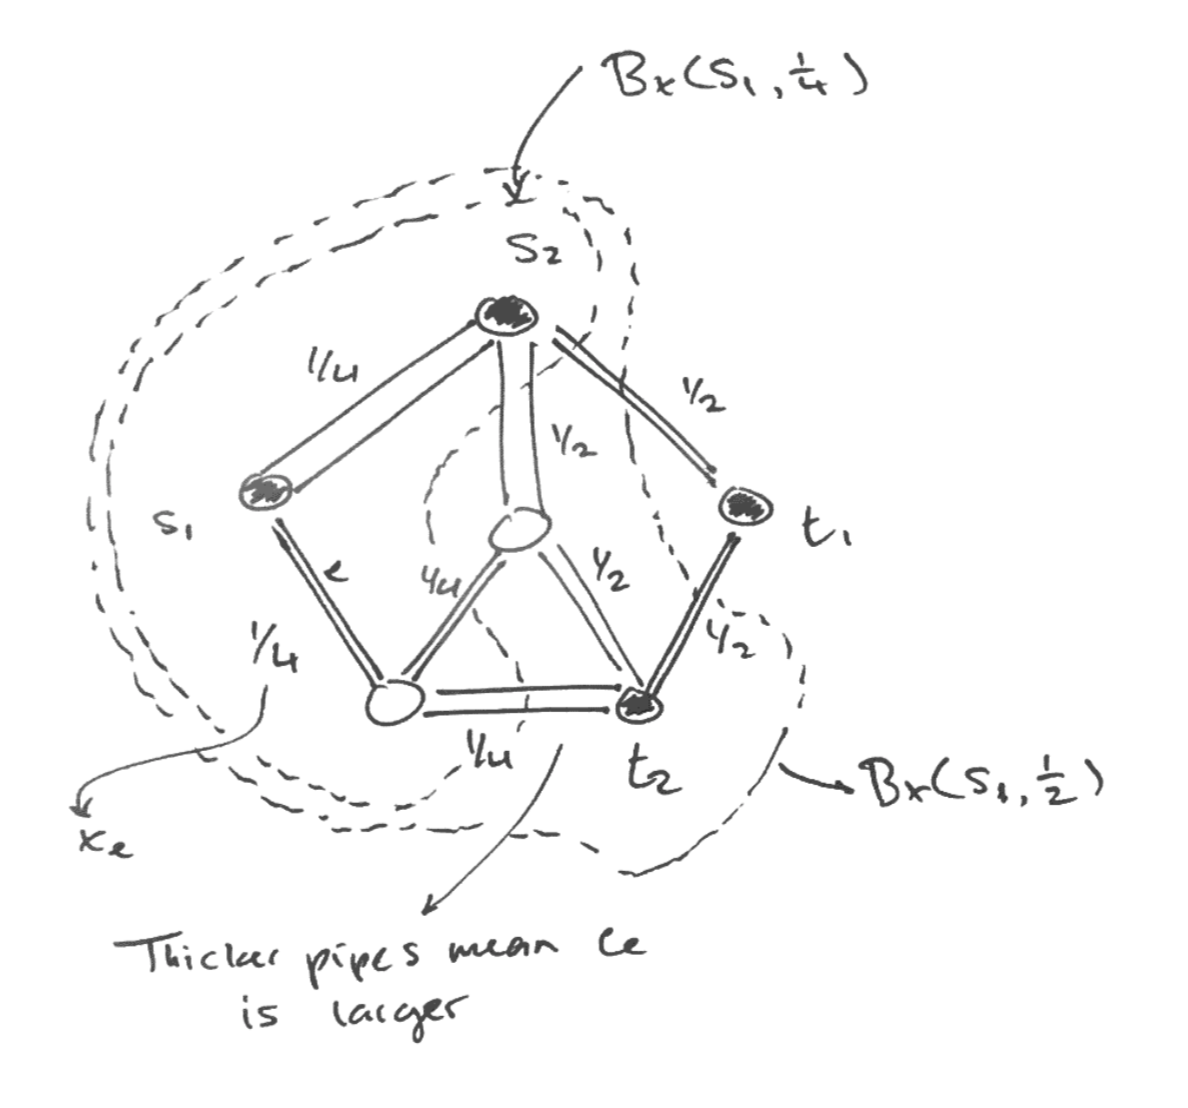
\includegraphics[scale=0.45]{images/image-1.png}
\end{figure}
\vspace{-1em}

Notice that $\mathcal{B}_x(s_1, \frac{1}{2})$ contains both $s_2$ and $t_2$. What is the largest value of $r$ such that a cluster centered at $s_i$ will not contain any $s_j, t_j$ pair? Because $d_x(s_i, t_i) \geq 1$ for any pair $s_i, t_i$, choosing $r < \frac{1}{2}$ suffices because of the triangle inequality. If there is a ball $\mathcal{B}_x(s_i, r)$ where $r < \frac{1}{2}$ containing any $s_j, t_j$, then
\begin{equation*}
x_{s_j, t_j}
= d_x(s_j, t_j)
\leq d_x(s_j, s_i) + d_x(s_i, t_j)
< \frac{1}{2} + \frac{1}{2}
= 1
\end{equation*}

contradicting the fact that $x_{s_j, t_j} \geq 1$. Consequently, any $r < \frac{1}{2}$ will lead the following rounding procedure to return a valid multicut. Notice that in the following procedure, we remove the ball of radius $r$ at each iteration to ensure that no edge is within two different balls.

\noindent\fbox {
\parbox{45.5em} {
\alglabel{alg:rounding}
\textbf{LP Rounding Algorithm}~\thealgorithm

Given $G = (V, E)$, source-sink pairs $\{ (s_i, t_i): i = 1, \ldots, k \}$ and radius $r \in [0, \frac{1}{2})$, do the following:

\begin{quote}
\begin{enumerate}[1.]
\item Solve the linear program relaxation~\ref{eq:metric-lp} for $x$ and set $F = \varnothing$.

\item For $i = 1, \ldots, k$ do:
\begin{enumerate}[-]
\item If $s_i, t_i$ are not separated in $(V, E - F)$, then choose $\mathcal{B}_x(s_i, r)$

\item Update $F = F \cup \partial(\mathcal{B}_x(s_i, r))$

\item Remove vertices in $\mathcal{B}_x(s_i, r)$ and edges in $E(\mathcal{B}_x(s_i, r)) \cup \partial (\mathcal{B}_x(s_i, r))$.
\end{enumerate}

\item Return $F$
\end{enumerate}
\end{quote}
}
}
\vspace{1em}

Now that we have a way of procuring a valid multicut, we can turn our attention towards making it low-cost. Our goal will now be to show that an auspicious choice of $r$ will allow us to bound the cost of the rounded multicut.
